\chapter{Relações (1º Bimestre)}

\section{Funções trigonométricas}

In the 3º bimestre of the 8ª série do Ensino Fundamental, we defined three
continuous functions $\tan$, $\cos$, $\sin$ on $(0,\frac{\pi}{2})$ as quotients
of sides inside rectangle triangles. We have ${\tan 0} = {\sin 0} = 0$,
${\cos 0} = 1$. Hence we were able to extended them to continuous functions on
$(-\frac{\pi}{2},\frac{\pi}{2})$ by claiming
$\cos{(-\alpha)} = \cos{(\alpha)}$, $\sin{(-\alpha)} = -\sin{(\alpha)}$ and
$\tan{(-\alpha)} = -\tan{(\alpha)}$.
We have $\lim_{\alpha \rightarrow {\left(\pm\frac{\pi}{2}\right)}^-} \tan \alpha =
\pm\infty$ but the corresponding limits for $\cos$ and $\sin$ are finite and
so we can define $\cos {-\frac{\pi}{2}} = \cos {\frac{\pi}{2}} = 0$,
$\sin {\frac{\pi}{2}} = 1$, $\sin {-\frac{\pi}{2}} = -1$.
Once we defined $\cos$ and $\sin$ on
$\left[-\frac{\pi}{2}, \frac{\pi}{2}\right]$ we can then extend them to
continuous functions on $\left[-\frac{\pi}{2}, \frac{3\pi}{2}\right]$
using the formulas $\cos{(\pi-\alpha)} = -\cos{(\alpha)}$ and
$\sin{(\pi-\alpha)} = \sin{(\alpha)}$. Finally, we extend $\cos, \sin$ to
$\mathbb R$ by making them $2\pi$-periodic and $\tan$ to
$\bigcup_{k \in \mathbb Z}
\left]{-\frac{\pi}{2} + k\pi}, {\frac{\pi}{2} +k\pi} \right[$ by making it
$\pi$-periodic.
    Note that the properties $\cos^2 \alpha + \sin^2 \alpha = 1$,
    $\cos\left(\frac{\pi}{2} - \alpha\right) = \sin \alpha$,
    $\sin\left(\frac{\pi}{2} - \alpha\right) = \cos \alpha$ and
$\tan \alpha = \frac{\sin \alpha}{\cos \alpha}$ that are verified for the
interpretation as quotients in rectangle triangle is also true for the
extensions of the functions.

We also saw that the values of the function for special angles. The following
table contains a summary for $-\pi < \alpha \leq \pi$ that can easily be
extended by periocity of the trigonometric functions.

    \begin{center}
  \begin{tabular}{| l | c | c | c | c | c | c | c | c | c | c | c | c | c | c | c | c |}
    \hline
    $\alpha$ &
    $-\frac{5\pi}{6}$ &
    $-\frac{3\pi}{4}$ &
    $-\frac{2\pi}{3}$ &
    $-\frac{\pi}{2}$ &
    $-\frac{\pi}{3}$ &
    $-\frac{\pi}{4}$ &
    $-\frac{\pi}{6}$ &
    $0$ &
    $\frac{\pi}{6}$ &
    $\frac{\pi}{4}$ &
    $\frac{\pi}{3}$ &
    $\frac{\pi}{2}$ &
    $\frac{2\pi}{3}$ &
    $\frac{3\pi}{4}$ &
    $\frac{5\pi}{6}$ &
    $\pi$ \\
    \hline
    $\sin \alpha$ &
    $-\frac{1}{2}$ &
    $-\frac{\sqrt{2}}{2}$ &
    $-\frac{\sqrt{3}}{2}$ &
    $-1$ &
    $-\frac{\sqrt{3}}{2}$ &
    $-\frac{\sqrt{2}}{2}$ &
    $-\frac{1}{2}$ &
    $0$ &
    $\frac{1}{2}$ &
    $\frac{\sqrt{2}}{2}$ &
    $\frac{\sqrt{3}}{2}$ &
    $1$ &
    $\frac{\sqrt{3}}{2}$ &
    $\frac{\sqrt{2}}{2}$ &
    $\frac{1}{2}$ &
    $0$
    \\
    \hline
    $\cos \alpha$ &
    $-\frac{\sqrt{3}}{2}$ &
    $-\frac{\sqrt{2}}{2}$ &
    $-\frac{1}{2}$ &
    $0$ &
    $\frac{1}{2}$ &
    $\frac{\sqrt{2}}{2}$ &
    $\frac{\sqrt{3}}{2}$ &
    $1$ &
    $\frac{\sqrt{3}}{2}$ &
    $\frac{\sqrt{2}}{2}$ &
    $\frac{1}{2}$ &
    $0$ &
    $-\frac{1}{2}$ &
    $-\frac{\sqrt{2}}{2}$ &
    $-\frac{\sqrt{3}}{2}$ &
    $-1$
    \\
    \hline
    $\tan \alpha$ &
    $\dots$ &
    $\dots$ &
    $\dots$ &
    $-\infty$ &
    $-\sqrt{3}$ &
    $-1$ &
    $-\frac{\sqrt{3}}{3}$ &
    $0$ &
    $\frac{\sqrt{3}}{3}$ &
    $1$ &
    $\sqrt{3}$ &
    $\infty$ &
    $\dots$ &
    $\dots$ &
    $\dots$ &
    $\dots$
    \\
    \hline
  \end{tabular}
  \end{center}

Here are the graphs of the trigonometric functions:

\begin{center}
  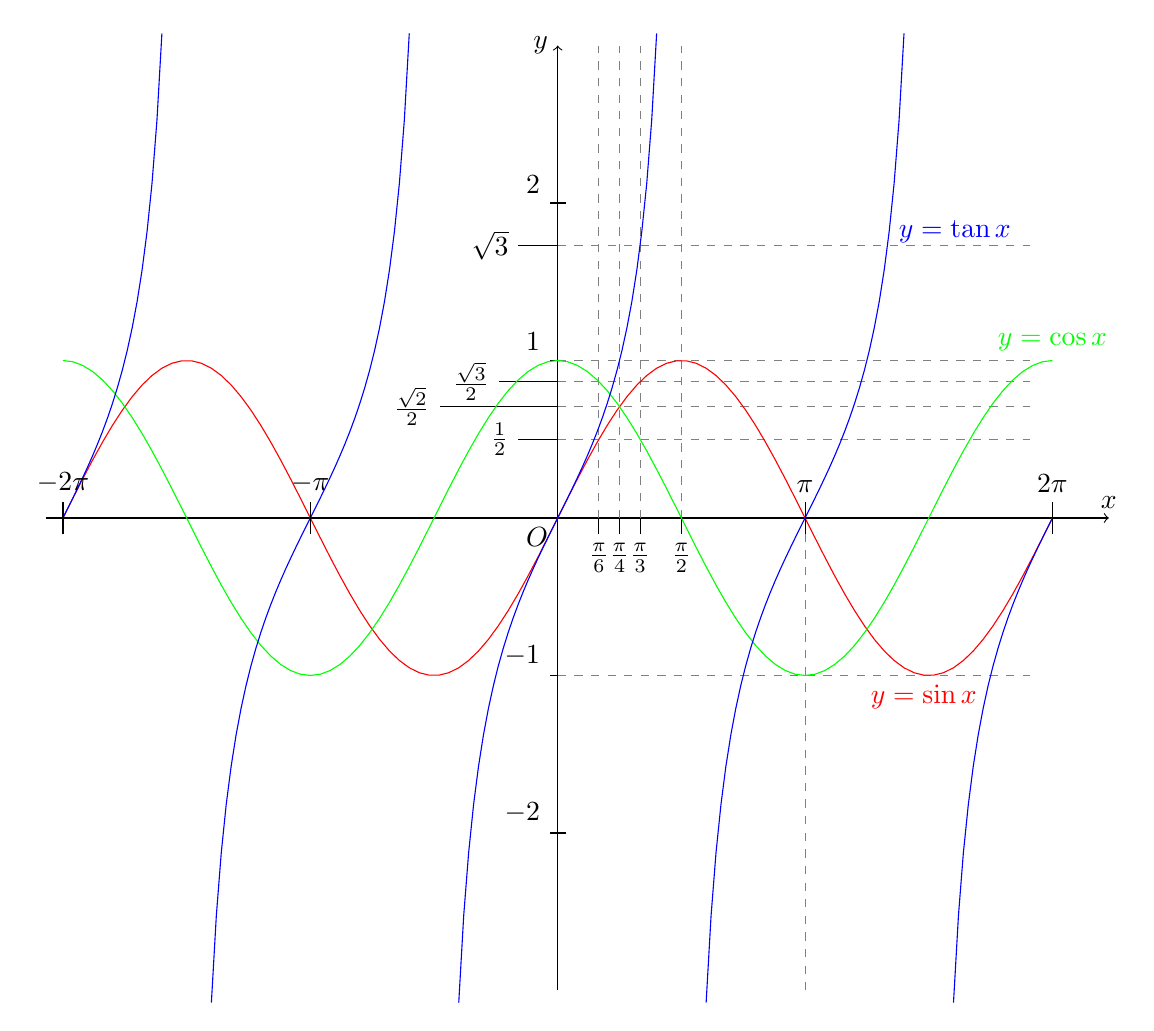
\begin{tikzpicture}[yscale=2]
    \begin{scope}
      \draw[->] (-6.5,0) -- (7,0) node[above] {$x$};
      \draw[->] (0,-3) -- (0,3) node[left] {$y$};;

      \draw[color=gray,style=dashed]
      (0.5235987755982988,0)--(0.5235987755982988,3);
      \draw(0.5235987755982988,0)--
      (0.5235987755982988,-.1) node[below]{$\frac{\pi}{6}$};
      \draw[color=gray,style=dashed]
      (0.7853981633974483,0)--(0.7853981633974483,3);
      \draw(0.7853981633974483,0)--
      (0.7853981633974483,-.1) node[below]{$\frac{\pi}{4}$};
      \draw[color=gray,style=dashed]
      (1.047197551196597,0)--(1.047197551196597,3);
      \draw(1.047197551196597,0)--
      (1.047197551196597,-.1) node[below]{$\frac{\pi}{3}$};
      \draw[color=gray,style=dashed]
      (1.570796326794896,0)--(1.570796326794896,3);
      \draw(1.570796326794896,0)--
      (1.570796326794896,-.1) node[below]{$\frac{\pi}{2}$};
      \draw[color=gray,style=dashed]
      (3.141592653589793,-3)--(3.141592653589793,0);

      \foreach \y in {-2,-1,1,2} {
        \draw(.1,\y) -- (-.1,\y) node[above left]{$\y$};
      }
      \draw[color=gray,style=dashed] (0,1)--(6,1) (0,-1) -- (6,-1);
      \draw[color=gray,style=dashed]
      (0,1.732050807568877)--(6,1.732050807568877);
      \draw(0,1.732050807568877)--(-.5,1.732050807568877)
      node[left]{$\sqrt{3}$};
      \draw[color=gray,style=dashed]
      (0,.5)--(6,.5);
      \draw(0,.5)--(-.5,.5) node[left]{$\frac{1}{2}$};

      \draw[color=gray,style=dashed]
      (0,0.8660254037844386)--(6,0.8660254037844386);
      \draw(0,0.8660254037844386)--(-.75,0.8660254037844386)
      node[left]{$\frac{\sqrt{3}}{2}$};


      \draw[color=gray,style=dashed]
      (0,0.7071067811865475)--(6,0.7071067811865475);
      \draw(0,0.7071067811865475)--(-1.5,0.7071067811865475)
      node[left]{$\frac{\sqrt{2}}{2}$};

      \draw[color=red] (-6.2832,0)--(-6.1575,0.1253)--(-6.0319,0.2487)--(-5.9062,0.3681)--(-5.7805,0.4818)--(-5.6549,0.5878)--(-5.5292,0.6845)--(-5.4035,0.7705)--(-5.2779,0.8443)--(-5.1522,0.9048)--(-5.0265,0.9511)--(-4.9009,0.9823)--(-4.7752,0.998)--(-4.6496,0.998)--(-4.5239,0.9823)--(-4.3982,0.9511)--(-4.2726,0.9048)--(-4.1469,0.8443)--(-4.0212,0.7705)--(-3.8956,0.6845)--(-3.7699,0.5878)--(-3.6442,0.4818)--(-3.5186,0.3681)--(-3.3929,0.2487)--(-3.2673,0.1253)--(-3.1416,0)--(-3.0159,-0.1253)--(-2.8903,-0.2487)--(-2.7646,-0.3681)--(-2.6389,-0.4818)--(-2.5133,-0.5878)--(-2.3876,-0.6845)--(-2.2619,-0.7705)--(-2.1363,-0.8443)--(-2.0106,-0.9048)--(-1.885,-0.9511)--(-1.7593,-0.9823)--(-1.6336,-0.998)--(-1.508,-0.998)--(-1.3823,-0.9823)--(-1.2566,-0.9511)--(-1.131,-0.9048)--(-1.0053,-0.8443)--(-0.8796,-0.7705)--(-0.754,-0.6845)--(-0.6283,-0.5878)--(-0.5027,-0.4818)--(-0.377,-0.3681)--(-0.2513,-0.2487)--(-0.1257,-0.1253)--(0,0)--(0.1257,0.1253)--(0.2513,0.2487)--(0.377,0.3681)--(0.5027,0.4818)--(0.6283,0.5878)--(0.754,0.6845)--(0.8796,0.7705)--(1.0053,0.8443)--(1.131,0.9048)--(1.2566,0.9511)--(1.3823,0.9823)--(1.508,0.998)--(1.6336,0.998)--(1.7593,0.9823)--(1.885,0.9511)--(2.0106,0.9048)--(2.1363,0.8443)--(2.2619,0.7705)--(2.3876,0.6845)--(2.5133,0.5878)--(2.6389,0.4818)--(2.7646,0.3681)--(2.8903,0.2487)--(3.0159,0.1253)--(3.1416,0)--(3.2673,-0.1253)--(3.3929,-0.2487)--(3.5186,-0.3681)--(3.6442,-0.4818)--(3.7699,-0.5878)--(3.8956,-0.6845)--(4.0212,-0.7705)--(4.1469,-0.8443)--(4.2726,-0.9048)--(4.3982,-0.9511)--(4.5239,-0.9823)--(4.6496,-0.998)node[below]{$y = \sin{x}$}--(4.7752,-0.998)--(4.9009,-0.9823)--(5.0265,-0.9511)--(5.1522,-0.9048)--(5.2779,-0.8443)--(5.4035,-0.7705)--(5.5292,-0.6845)--(5.6549,-0.5878)--(5.7805,-0.4818)--(5.9062,-0.3681)--(6.0319,-0.2487)--(6.1575,-0.1253)--(6.2832,0);
      \draw[color=green] (-6.2832,1)--(-6.1575,0.9921)--(-6.0319,0.9686)--(-5.9062,0.9298)--(-5.7805,0.8763)--(-5.6549,0.809)--(-5.5292,0.729)--(-5.4035,0.6374)--(-5.2779,0.5358)--(-5.1522,0.4258)--(-5.0265,0.309)--(-4.9009,0.1874)--(-4.7752,0.0628)--(-4.6496,-0.0628)--(-4.5239,-0.1874)--(-4.3982,-0.309)--(-4.2726,-0.4258)--(-4.1469,-0.5358)--(-4.0212,-0.6374)--(-3.8956,-0.729)--(-3.7699,-0.809)--(-3.6442,-0.8763)--(-3.5186,-0.9298)--(-3.3929,-0.9686)--(-3.2673,-0.9921)--(-3.1416,-1)--(-3.0159,-0.9921)--(-2.8903,-0.9686)--(-2.7646,-0.9298)--(-2.6389,-0.8763)--(-2.5133,-0.809)--(-2.3876,-0.729)--(-2.2619,-0.6374)--(-2.1363,-0.5358)--(-2.0106,-0.4258)--(-1.885,-0.309)--(-1.7593,-0.1874)--(-1.6336,-0.0628)--(-1.508,0.0628)--(-1.3823,0.1874)--(-1.2566,0.309)--(-1.131,0.4258)--(-1.0053,0.5358)--(-0.8796,0.6374)--(-0.754,0.729)--(-0.6283,0.809)--(-0.5027,0.8763)--(-0.377,0.9298)--(-0.2513,0.9686)--(-0.1257,0.9921)--(0,1)--(0.1257,0.9921)--(0.2513,0.9686)--(0.377,0.9298)--(0.5027,0.8763)--(0.6283,0.809)--(0.754,0.729)--(0.8796,0.6374)--(1.0053,0.5358)--(1.131,0.4258)--(1.2566,0.309)--(1.3823,0.1874)--(1.508,0.0628)--(1.6336,-0.0628)--(1.7593,-0.1874)--(1.885,-0.309)--(2.0106,-0.4258)--(2.1363,-0.5358)--(2.2619,-0.6374)--(2.3876,-0.729)--(2.5133,-0.809)--(2.6389,-0.8763)--(2.7646,-0.9298)--(2.8903,-0.9686)--(3.0159,-0.9921)--(3.1416,-1)--(3.2673,-0.9921)--(3.3929,-0.9686)--(3.5186,-0.9298)--(3.6442,-0.8763)--(3.7699,-0.809)--(3.8956,-0.729)--(4.0212,-0.6374)--(4.1469,-0.5358)--(4.2726,-0.4258)--(4.3982,-0.309)--(4.5239,-0.1874)--(4.6496,-0.0628)--(4.7752,0.0628)--(4.9009,0.1874)--(5.0265,0.309)--(5.1522,0.4258)--(5.2779,0.5358)--(5.4035,0.6374)--(5.5292,0.729)--(5.6549,0.809)--(5.7805,0.8763)--(5.9062,0.9298)--(6.0319,0.9686)--(6.1575,0.9921)--(6.2832,1) node[above] {$y=\cos x$};
      \draw[color=blue]
      (-6.2832,0)--(-6.2204,0.0629)--(-6.1575,0.1263)--(-6.0947,0.1908)--(-6.0319,0.2568)--(-5.969,0.3249)--(-5.9062,0.3959)--(-5.8434,0.4706)--(-5.7805,0.5498)--(-5.7177,0.6346)--(-5.6549,0.7265)--(-5.592,0.8273)--(-5.5292,0.9391)--(-5.4664,1.0649)--(-5.4035,1.2088)--(-5.3407,1.3764)--(-5.2779,1.5757)--(-5.215,1.819)--(-5.1522,2.1251)--(-5.0894,2.5257)--(-5.0265,3.0777)
      (-4.3982,-3.0777)--(-4.3354,-2.5257)--(-4.2726,-2.1251)--(-4.2097,-1.819)--(-4.1469,-1.5757)--(-4.0841,-1.3764)--(-4.0212,-1.2088)--(-3.9584,-1.0649)--(-3.8956,-0.9391)--(-3.8327,-0.8273)--(-3.7699,-0.7265)--(-3.7071,-0.6346)--(-3.6442,-0.5498)--(-3.5814,-0.4706)--(-3.5186,-0.3959)--(-3.4558,-0.3249)--(-3.3929,-0.2568)--(-3.3301,-0.1908)--(-3.2673,-0.1263)--(-3.2044,-0.0629)--(-3.1416,0)--(-3.0788,0.0629)--(-3.0159,0.1263)--(-2.9531,0.1908)--(-2.8903,0.2568)--(-2.8274,0.3249)--(-2.7646,0.3959)--(-2.7018,0.4706)--(-2.6389,0.5498)--(-2.5761,0.6346)--(-2.5133,0.7265)--(-2.4504,0.8273)--(-2.3876,0.9391)--(-2.3248,1.0649)--(-2.2619,1.2088)--(-2.1991,1.3764)--(-2.1363,1.5757)--(-2.0735,1.819)--(-2.0106,2.1251)--(-1.9478,2.5257)--(-1.885,3.0777)
      (-1.2566,-3.0777)--(-1.1938,-2.5257)--(-1.131,-2.1251)--(-1.0681,-1.819)--(-1.0053,-1.5757)--(-0.9425,-1.3764)--(-0.8796,-1.2088)--(-0.8168,-1.0649)--(-0.754,-0.9391)--(-0.6912,-0.8273)--(-0.6283,-0.7265)--(-0.5655,-0.6346)--(-0.5027,-0.5498)--(-0.4398,-0.4706)--(-0.377,-0.3959)--(-0.3142,-0.3249)--(-0.2513,-0.2568)--(-0.1885,-0.1908)--(-0.1257,-0.1263)--(-0.0628,-0.0629)--(0,0)--(0.0628,0.0629)--(0.1257,0.1263)--(0.1885,0.1908)--(0.2513,0.2568)--(0.3142,0.3249)--(0.377,0.3959)--(0.4398,0.4706)--(0.5027,0.5498)--(0.5655,0.6346)--(0.6283,0.7265)--(0.6912,0.8273)--(0.754,0.9391)--(0.8168,1.0649)--(0.8796,1.2088)--(0.9425,1.3764)--(1.0053,1.5757)--(1.0681,1.819)--(1.131,2.1251)--(1.1938,2.5257)--(1.2566,3.0777)
      (1.885,-3.0777)--(1.9478,-2.5257)--(2.0106,-2.1251)--(2.0735,-1.819)--(2.1363,-1.5757)--(2.1991,-1.3764)--(2.2619,-1.2088)--(2.3248,-1.0649)--(2.3876,-0.9391)--(2.4504,-0.8273)--(2.5133,-0.7265)--(2.5761,-0.6346)--(2.6389,-0.5498)--(2.7018,-0.4706)--(2.7646,-0.3959)--(2.8274,-0.3249)--(2.8903,-0.2568)--(2.9531,-0.1908)--(3.0159,-0.1263)--(3.0788,-0.0629)--(3.1416,0)--(3.2044,0.0629)--(3.2673,0.1263)--(3.3301,0.1908)--(3.3929,0.2568)--(3.4558,0.3249)--(3.5186,0.3959)--(3.5814,0.4706)--(3.6442,0.5498)--(3.7071,0.6346)--(3.7699,0.7265)--(3.8327,0.8273)--(3.8956,0.9391)--(3.9584,1.0649)--(4.0212,1.2088)--(4.0841,1.3764)--(4.1469,1.5757)--(4.2097,1.819)node[right]{$y=\tan x$}--(4.2726,2.1251)--(4.3354,2.5257)--(4.3982,3.0777)
      (5.0265,-3.0777)--(5.0894,-2.5257)--(5.1522,-2.1251)--(5.215,-1.819)--(5.2779,-1.5757)--(5.3407,-1.3764)--(5.4035,-1.2088)--(5.4664,-1.0649)--(5.5292,-0.9391)--(5.592,-0.8273)--(5.6549,-0.7265)--(5.7177,-0.6346)--(5.7805,-0.5498)--(5.8434,-0.4706)--(5.9062,-0.3959)--(5.969,-0.3249)--(6.0319,-0.2568)--(6.0947,-0.1908)--(6.1575,-0.1263)--(6.2204,-0.0629)--(6.2832,0);

      \draw(-3.141592653589793,-.1)--(-3.141592653589793,.1) node[above]{$-\pi$};
      \draw(-6.283185307179586,-.1)--(-6.283185307179586,.1) node[above]{$-2\pi$};
      \draw(3.141592653589793,-.1)--(3.141592653589793,.1) node[above]{$\pi$};
      \draw(6.283185307179586,-.1)--(6.283185307179586,.1) node[above]{$2\pi$};
      \draw(0,0) node[below left] {$O$};


    \end{scope}
  \end{tikzpicture}
\end{center}

We note that $\tan$ is strictly increasing on
$\left(-\frac{\pi}{2}, \frac{\pi}{2}\right)$ and with limits $\pm \infty$
at the bounds. Hence we can define an inverse function $\arctan$ on $\mathbb R$
by saying that $\arctan x = \alpha$ where $\alpha$ is the unique
$\alpha \in \left(-\frac{\pi}{2}, \frac{\pi}{2}\right)$ such that
$x = \tan \alpha$. Similarly, we can define two functions $\arccos x$
(respectively $\arcsin x$) on $[-1,1]$ as respectively
the unique $0 \leq x \leq \pi$ such that
$\cos \alpha = x$ (respectively the unique $-\pi/2 \leq x \leq \pi$ such that
$\sin \alpha = x$). As for $\log$, the graphs of these inverse functions and
be obtained using a symmetry along the line $y = x$ and in particular the
functions are continuous.

Actually, in the 8ª série do Ensino Fundamental we also defined the inverse
trigonometric functions using rectangle triangles of sides $1, x$ where
$0 \leq x \leq 1$. This allows to deduce more properties that can be verified
for the extended functions as well.
For example, suppose that the hypotenus is
$\sqrt{1+x^2}$ (and so $1,x$ the other sides).
$\tan {\arctan x} = x = \frac{x}{1}$ is clear by definition and so
$\arctan x$ is the angle adjacent to the side of length $1$. Hence
we also have $\cos \left( \arctan x \right) =  \frac{1}{\sqrt{1+x^2}}$
and $\sin \left( \arctan x \right) =  \frac{x}{\sqrt{1+x^2}}$.

For any $\alpha, \beta$ we have can prove (see Exercício 1) that
$$
\sin\left(\alpha \pm \beta\right) =
{\sin \alpha \cos \beta} \pm {\cos \alpha \sin \beta}
$$
$$
\cos\left(\alpha \pm \beta\right) =
{\cos \alpha \cos \beta} \mp {\sin \alpha \sin \beta}
$$
and in particular if $\beta = \alpha$:
$$
\sin\left(2\alpha\right) =
2{\sin \alpha \cos \alpha}
$$
$$
\cos\left(2\alpha\right) =
         {\cos^2 \alpha} - {\sin^2 \alpha} =
         2{\cos^2 \alpha} - 1 = 1 - 2{\sin^2 \alpha}
$$
The last one can be rewritten as
$$
\sin^2 \alpha = \frac{1-\cos{(2\alpha)}}{2}
$$
$$
\cos^2 \alpha = \frac{1+\cos{(2\alpha)}}{2}
$$
Also, when well-defined we have
$\tan\left(\alpha \pm \beta\right) =
\frac{\sin\left(\alpha \pm \beta\right)}{\cos\left(\alpha \pm \beta\right)}=
\frac{{\sin \alpha \cos \beta} \pm {\cos \alpha \sin \beta}}
     {{\cos \alpha \cos \beta} \mp {\sin \alpha \sin \beta}}
     $ and dividing the numerator and denominator by
     ${\cos \alpha \cos \beta}$ we obtain
$$
\tan\left(\alpha \pm \beta\right) =
\frac{\tan \alpha \pm \tan \beta}{1 \mp {\tan \alpha \tan \beta}}
$$
from which we deduce
$$
\tan\left(2\alpha\right) =
\frac{2\tan \alpha}{1 - {\tan^2 \alpha}}
$$
and for any $x,y$
$$
\arctan{x} \pm \arctan{y} = \arctan \left(\frac{x\pm y}{1 \mp xy}\right)
$$
The following properties can easily be proved by expanding the
right hand side using the angle addition properties stated above:
$$
\cos \alpha \cos \beta =
\frac{\cos\left(\alpha - \beta\right) + \cos\left(\alpha + \beta\right)}{2}
$$
$$
\sin \alpha \sin \beta =
\frac{\cos\left(\alpha - \beta\right) - \cos\left(\alpha + \beta\right)}{2}
$$
$$
\sin \alpha \cos \beta =
\frac{\sin\left(\alpha + \beta\right) + \sin\left(\alpha - \beta\right)}{2}
$$
$$
\cos \alpha \sin \beta =
\frac{\sin\left(\alpha + \beta\right) - \sin\left(\alpha - \beta\right)}{2}
$$
We then immediately deduce
$$
\tan \alpha \tan \beta =
\frac{\sin \alpha \sin \beta}{\cos \alpha \cos \beta} =
\frac{\cos\left(\alpha - \beta\right) - \cos\left(\alpha + \beta\right)}
{\cos\left(\alpha - \beta\right) + \cos\left(\alpha + \beta\right)}$$
and
$$\sin \alpha \pm \sin \beta = 2 \sin\left( \frac{\alpha \pm \beta}{2} \right) \cos\left( \frac{\alpha \mp \beta}{2} \right)$$
$$\cos \alpha + \cos \beta = 2 \cos\left( \frac{\alpha + \beta} {2} \right) \cos\left( \frac{\alpha - \beta}{2} \right)$$
$$\cos \alpha - \cos \beta = -2\sin\left( {\alpha + \beta \over 2}\right) \sin\left({\alpha - \beta \over 2}\right)$$

\subsection*{Exercício 1}

In this exercise, we want to prove the formulas
$$
\sin\left(\alpha + \beta\right) =
{\sin \alpha \cos \beta} + {\cos \alpha \sin \beta}
$$
$$
\cos\left(\alpha + \beta\right) =
{\cos \alpha \cos \beta} - {\sin \alpha \sin \beta}
$$
for any $\alpha, \beta$.

\begin{enumerate}
\item Verify the formulas if $\alpha = 0$ or $\beta = 0$.
\item Verify the formulas if $\alpha = \pm\frac{\pi}{2}$ or
  $\beta = \pm\frac{\pi}{2}$.
\item Verify the formulas if $\alpha = \pm\pi$ or $\beta = \pm\pi$.
\item Verify the formulas if $\alpha + \beta = 0$.
\item Verify the formulas if $\alpha + \beta = \pm\frac{\pi}{2}$.
\item Verify the formulas if $\alpha + \beta = \pm\pi$.
\item Prove that if the formulas hold for $(\alpha, \beta)$ then they also hold
  for $(-\alpha, -\beta)$.
\item Prove that if the formulas hold for $(\alpha, \beta)$ the they also hold
  for $(\alpha\pm\pi, \beta)$ and $(\alpha, \beta\pm\pi)$
\item We now consider two acute angles $0 < \alpha, \beta < \frac{\pi}{2}$
  such that $\alpha + \beta < \frac{\pi}{2}$.
Let $\mathcal R$ uma reta and $O \in \mathcal R$. We consider a point
$A$ such that $OA = 1$ and the angle between $\mathcal R$ and $(OA)$ is
$\alpha+\beta$. Let $B$ such that $(OB) \perp \mathcal R$ and
$OBA$ is rectangle in $B$. Let $C$ such that
$\text{angle}\left(\mathcal R, (OC)\right) = \alpha$,
$\text{angle}\left((OC), (OA)\right) = \beta$ and
$OAC$ is rectangle in $C$. Let $D \in \mathcal R$ such that $OCD$ is rectangle
in $D$. Finally, let $E$ be the intersection of $(AB)$ and $(CD)$.
Draw a schema.
\item Express $CA$ and $CO$ in function of $\beta$.
\item Express $DC$ and $DO$ in function of $\alpha, \beta$.
\item What are the internal angles of the triangle $OAB$?
\item Deduce an expression of $BA$ and $BO$ in function of $\alpha, \beta$.
\item What are the internal angles of the triangle $AEC$?
\item Deduce an expression of $EC$ and $EA$ in function of $\alpha, \beta$.
\item Express $BA$ in function of $EA$ and $DO$ and deduce the addition formula
  for $\cos$.
\item Express $BO$ in function of $DC$ and $CE$ and deduce the addition formula
  for $\sin$.
\item We still consider acute angles $0 < \alpha, \beta < \frac{\pi}{2}$
  but assume that $\frac{\pi}{2} < \alpha+\beta$. Draw a schema
  and verify that a similar proof holds.
\item Deduce that the formulas also hold for any
  $-\frac{\pi}{2} < \alpha, \beta < 0$.
\item We now consider $-\frac{\pi}{2} < \beta < 0 < \alpha < \frac{\pi}{2}$
  such that $0 < \alpha+\beta$.
  If we consider non-oriented angle, we must modify the construction to take
  $\text{angle}\left((OC), (OA)\right) = {|\beta|} = -\beta$.
  Draw a schema and verify that a similar proof holds.
\item Deduce that the formulas also hold
  if $-\frac{\pi}{2} < \beta < 0 < \alpha < \frac{\pi}{2}$ and
  $\alpha+\beta < 0$.
\item Conclude that the formulas hold for any $\alpha, \beta$. What can you say
  about $\sin\left(\alpha - \beta\right)$ and
  $\cos\left(\alpha - \beta\right)$?
\end{enumerate}

\subsection*{Exercício 2}

\begin{enumerate}
\item Use your calculator to complete the following table with
  approximate values and use it to draw the graph of the seno function on
  the interval $[-\pi, \pi]$.
    \begin{center}
    \begin{tabular}{| c | c | }
      \hline
      $x$ & $\sin{(x)}$ \\
      \hline
      $0$ & \\
      $0.15$ & \\
      $0.3$ & \\
      $0.45$ & \\
      $\frac{\pi}{6}$ & \\
      $0.60$ & \\
      $0.75$ & \\
      $0.90$ & \\
      $1.05$ & \\
      $1.20$ & \\
      $1.35$ & \\
      $\frac{\pi}{2}$ & \\
      \hline
    \end{tabular}
  \end{center}

\item
  We consider the function $f(x) = 2 \sin{(3x)} + 5$ for all
  $x \in \mathbb R$.
  Show that $f$ is $\frac{2\pi}{3}$-periodic.
\item Show that the point $(0,5)$ is a center of symmetry for the graph of $f$.
\item Verify that the reta
  $x = \frac{\pi}{3}$ is an axis of symmetry of the graph of $f$.

\item Use your calculator to complete the following table with
  approximate values and use it to draw the graph of $f$.
  \begin{center}
    \begin{tabular}{| c | c | c | c | }
      \hline
      $x$ & $\sin{(3x)}$ & $2\sin{(3x)}$ & $f(x) = 2\sin{(3x)}+5$ \\
      \hline
      $0$ & & & \\
      $0.05$ & & & \\
      $0.1$ & & & \\
      $0.15$ & & & \\
      $\frac{\pi}{18}$ & & & \\
      $0.20$ & & & \\
      $0.25$ & & & \\
      $0.30$ & & & \\
      $0.35$ & & & \\
      $0.40$ & & & \\
      $0.45$ & & & \\
      $\frac{\pi}{6}$ & & & \\
      \hline
    \end{tabular}
  \end{center}

\item Explain how to obtain the graph of $f$ from the graph of $\sin$.
\end{enumerate}

\subsection*{Exercício 3}

The voltage of an alternative current of frequency $f$ (in Hertz) and amplitude
$V_0$ (in volts) is a periodic function of the time $t$ (in seconds)
expressed as
%%
$$
{V(t)} = V_0 \sin\left(2 \pi f t\right)
$$
%%
The frequency used in Brazil for providing electrical power is
$f = 60\text{Hz}$. However, depending on the area, the root mean square voltage
$\frac{V_0}{\sqrt{2}}$ might be $127\text{V}$ or $220\text{V}$.

\begin{enumerate}
\item Verify that the alternative current in Brazil is $T$-periodic where
  $T = \frac{1}{60} \text{s} \approx 0.017\text{s}$.
\item Determine the possible amplitudes $V_0$ of alternative current in Brazil.
\item Draw the graphs of $V(t)$ for these two possible values of $V_0$.
\item When do we have $V(t) \geq 200 \text{V}$?
\item Before 1978, many areas used the frequency $f' = 50\text{Hz}$. How would
  that modify the graph of $V(t)$?
\end{enumerate}

\subsection*{Exercício 4}

We consider an ``idealized'' pendulum of length $l=1\text{m}$ with initial angle
$\theta_0 = 10°$ as shown on the following schema.
We suppose that the pivot $O$ is fixed at height $h = 2m$.

\begin{center}
  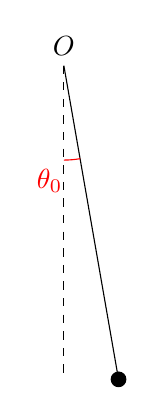
\begin{tikzpicture}[scale=4]

    \draw (0,0) node[above]{$O$} -- (0.1736481776669303, -0.9961946980917455);
    \fill (0.1736481776669303, -0.9961946980917455) circle(.025);
    \draw[style=dashed] (0,0) -- (0,-1);
    \draw[color=red](0,-.3) arc(-90:-85:.3) node[below left]{$\theta_0$}
         arc(-85:-80:.3);
  \end{tikzpicture}
\end{center}

The pendulum oscillates in such a way that the angle at time $t$ (in
seconds) is $\theta{(t)} = 10 \cos\left(\omega t\right)°$ where
$\omega \approx 3.13 \text{s}^{-1}$

\begin{enumerate}
\item What is the period of the pendulum oscillation?
\item When does the bob of the pendulum reach its maximum altitude?
\item When does the bob of the pendulum reach its minimum altitude?
\item For which value of $\theta(t)$ is the bob at altitude less
  than $1.0038 \text{m}$?
\item When does it happen?
\end{enumerate}

\subsection*{Exercício 5}

Solve the following equations:

\begin{enumerate}
\item $4 \cos^2{u} = 3$
\item $2\sin{v-1} = -\sqrt{2}$
\item $\sin{(3r+2)} = 1$
\item $3 \cos{(q-1)} = -7$
\item $3 \tan{(h-1)} = -7$
\item $\tan^2{y} + {(1-\sqrt{3})} \tan{y} = \sqrt{3}$
\item $\sin{(3x)} +  \sin x = \sqrt{3} \cos{x}$
\item $\cos{(5t)} = \cos{(3t)}  + \sin{t}$
\item $\cos{(2d)} + 2 = \cos{(d)} \left(\cos{(d)} + 2\right)$
\end{enumerate}

\subsection*{Exercício 6}

Solve the following inequations:

\begin{enumerate}
  \item $3 \sin{(u^2-8)} \leq 4$
  \item $6 \cos{(3x - 7)} < -3$
  \item $4 \sin^{2}{t} > 2$
  \item $5 \cos{(v+1)} < -7$
  \item $\tan{(y^2-7)} \geq 1$
  \item $\tan{y}\left(\tan{y} + 2\right) \leq 63$
\end{enumerate}

\section{Solução do Exercícios}

\subsection*{Exercício 1}

\begin{enumerate}
\item For example if $\alpha = 0$, we obtain
  $\cos\left(\alpha+\beta\right) = \cos \beta$
  and $\cos \alpha \cos \beta - \sin \alpha \sin \beta = 1 \times \cos \beta
  - 0 \times \sin \beta = \cos \beta$.
  We also have
  $\sin\left(\alpha+\beta\right) = \sin \beta$ and
  $\sin \alpha \cos \beta + \cos \alpha \sin \beta  =
  0 \times \cos \beta + 1 \times \sin \beta = \sin \beta$.

\item For example if $\alpha = \frac{\pi}{2}$, we obtain
  $\cos\left(\alpha+\beta\right) = -\sin \beta$
  and $\cos \alpha \cos \beta - \sin \alpha \sin \beta = 0 \times \cos \beta
  - 1 \times \sin \beta = -\sin \beta$.
  We also have
  $\sin\left(\alpha+\beta\right) = \cos \beta$ and
  $\sin \alpha \cos \beta + \cos \alpha \sin \beta  =
  1 \times \cos \beta + 0 \times \sin \beta = \cos \beta$.

\item For example if $\alpha = \pi$, we obtain
  $\cos\left(\alpha+\beta\right) = -\cos \beta$
  and $\cos \alpha \cos \beta - \sin \alpha \sin \beta = -1 \times \cos \beta
  - 0 \times \sin \beta = -\cos \beta$.
  We also have
  $\sin\left(\alpha+\beta\right) = -\sin \beta$ and
  $\sin \alpha \cos \beta + \cos \alpha \sin \beta  =
  0 \times \cos \beta -1 \times \sin \beta = -\sin \beta$.

\item If $\alpha + \beta = 0$ then
  $\cos\left(\alpha+\beta\right) = 1$
  and $\cos \alpha \cos \beta - \sin \alpha \sin \beta =
  \cos \alpha \cos \left(- \alpha \right)
  - \sin \alpha \sin \left(- \alpha \right) =
  \cos^2 \alpha + \sin^2 \alpha = 1$.
  Also,
  $\sin\left(\alpha+\beta\right) = 0$ and
  $\sin \alpha \cos \beta + \cos \alpha \sin \beta  =
  \sin \alpha \cos \left( - \alpha \right) + \cos \alpha
  \sin \left(- \alpha \right) =
  \sin \alpha \cos \alpha - \cos \alpha \sin \alpha = 0$.

\item For example if $\alpha+\beta = \frac{\pi}{2}$ then
  $\cos\left(\alpha+\beta\right) = 0$
  and $\cos \alpha \cos \beta - \sin \alpha \sin \beta =
  \cos \alpha \cos \left(\frac{\pi}{2} - \alpha \right)
  - \sin \alpha \sin \left(\frac{\pi}{2} - \alpha \right) =
  \cos \alpha \sin \alpha - \sin \alpha \cos \alpha = 0$.
  Also,
  $\sin\left(\alpha+\beta\right) = 1$ and
  $\sin \alpha \cos \beta + \cos \alpha \sin \beta  =
  \sin \alpha \cos \left(\frac{\pi}{2} - \alpha \right) + \cos \alpha
  \sin \left(\frac{\pi}{2} - \alpha \right) = \sin^2 \alpha + \cos^2 \alpha =
  1$.

\item For example if $\alpha + \beta = \pi$ then
  $\cos\left(\alpha+\beta\right) = -1$
  and $\cos \alpha \cos \beta - \sin \alpha \sin \beta =
  \cos \alpha \cos \left(\pi - \alpha \right)
  - \sin \alpha \sin \left(\pi - \alpha \right) =
  -\cos^2 \alpha - \sin^2 \alpha = -1$.
  Also,
  $\sin\left(\alpha+\beta\right) = 0$ and
  $\sin \alpha \cos \beta + \cos \alpha \sin \beta  =
  \sin \alpha \cos \left(\pi - \alpha \right) + \cos \alpha
  \sin \left(\pi - \alpha \right) =
  -\sin \alpha \cos \alpha + \cos \alpha \sin \alpha = 0$.

\item Changing the sign of $\alpha,\beta$ also change the sign of
  $\alpha+\beta$. Then for any
  $x \in \left\{ \alpha, \beta, {\alpha+\beta} \right\}$,
  $\sin{-x} = -\sin x$ and $\cos{-x} = \cos x$, from which the result is
  obvious.

\item For example replacing $\alpha$ with $\alpha+\pi$ also replaces
  $\alpha+\beta$ with $\alpha+\beta+\pi$. Then for any
  $x \in \left\{ \alpha, \beta, {\alpha+\beta} \right\}$,
  $\sin{x+\pi} = -\sin x$ and $\cos{x+\pi} = -\cos x$, from which the result is
  obvious.

\item We have the following schema:

  \begin{center}
    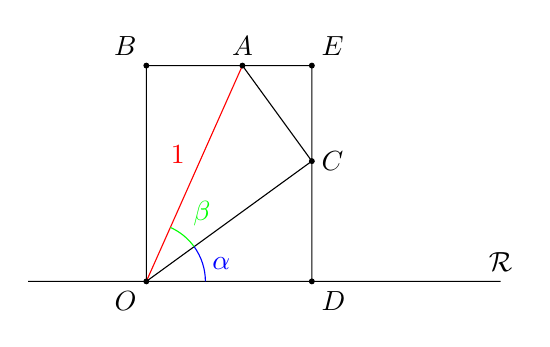
\begin{tikzpicture}
      \begin{scope}[scale=3]
        \draw (-.5,0) -- (1.5,0) node[above]{$\mathcal R$}
        (0.7006292692220367,0) -- (0.7006292692220367,0.9135454576426009)
        (0,0) -- (0.7006292692220367,0.5090369604551271)
        (0,0) -- (0,0.9135454576426009) --
        (0.7006292692220367,0.9135454576426009)
        (0.4067366430758004,0.9135454576426009) --
        (0.7006292692220367,0.5090369604551271)
        ;

        \draw[color=red]
        (0,0) --
        (0.2033683215379002,0.4567727288213004) node[above left] {$1$} --
        (0.4067366430758004,0.9135454576426009)
        ;

        \draw[fill]
        (0,0) node[below left] {$O$} circle(.01)
        (0.7006292692220367,0)
        node[below right] {$D$} circle(.01)
        (0.7006292692220367,0.5090369604551271)
        node[right] {$C$} circle(.01)
        (0,0.9135454576426009)
        node[above left] {$B$} circle(.01)
        (0.7006292692220367,0.9135454576426009)
        node[above right] {$E$} circle(.01)
        (0.4067366430758004,0.9135454576426009)
        node[above] {$A$} circle(.01)
        ;

        \draw[color=green]
        (0.2022542485937368,0.1469463130731182)
        arc(36:51:.25) node[above right]{$\beta$} arc(51:66:.25);

        \draw[color=blue]
        (.25,0) arc(0:18:.25) node[right]{$\alpha$} arc(18:36:.25);


      \end{scope}
 \end{tikzpicture}
\end{center}

\item In the triangle $OCA$ rectangle in $C$ we have
  $CO = OA \cos \widehat{O} = \cos \beta$ ;
  $CA = OA \sin \widehat{O} = \sin \beta$.
\item In the triangle $ODC$ rectangle in $D$ we have
  $DO = CO \widehat{O} = \cos \alpha \cos \beta$ and
  $DC = CO \widehat{O} = \sin \alpha \cos \beta$.
\item The triangle $OAB$ is rectangle in $B$ so $\widehat{B} = \frac{\pi}{2}$.
  $(OB) \perp \mathcal R$ and
  $\text{angle}\left(\mathcal R, (OA)\right) = \alpha+\beta$
  so $\widehat{O} = \frac{\pi}{2} - \alpha - \beta$. Finally,
  $\widehat{A} = \pi - \widehat{O} - \widehat{B} = \alpha + \beta$.
\item In the triangle $OAB$ rectangle in $B$ we have
  $BA = OA \cos \widehat{A} = \cos\left(\alpha+\beta\right)$
  and
  $BO = OA \sin \widehat{A} = \sin\left(\alpha+\beta\right)$.
\item $(OB) \perp \mathcal R$,
  $OBA$ is rectangle in $A$ and $OCD$ is rectangle in $D$ so
  $AEC$ is rectangle in $E$ and so $\widehat{E} = \frac{\pi}{2}$.
  The internals angle at vertex $A$ is
  $\alpha+\beta$ in the triangle $OAB$ and $\frac{\pi}{2} - \beta$ in
  the triangle $OCA$ so it is
  $\widehat{A} = \pi - \left(\alpha+\beta\right) -
  \left(\frac{\pi}{2} - \beta\right) = \frac{\pi}{2} - \alpha$ in
  the triangle $AEC$. We deduce that
  $\widehat{C} = \pi - \widehat{A} - \widehat{E} = \alpha$.
\item In the triangle $AEC$ rectangle in $E$ we have
  $CE = CA \cos \widehat{C} = \cos \alpha \sin \beta$ ;
  $EA = CA \sin \widehat{C} = \sin \alpha \sin \beta$.
\item By contruction,
  $BA = DO - EA$ and so
  $\cos\left(\alpha+\beta\right) =
  \cos \alpha \cos \beta -
  \sin \alpha \sin \beta$.
\item By contruction,
  $BO = DC + CE$ and so
  $\sin\left(\alpha+\beta\right) =
  \sin \alpha \cos \beta + \cos \alpha \sin \beta$
\item The schema becomes
  \begin{center}
    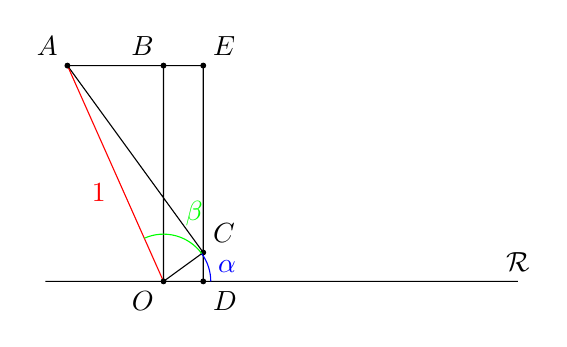
\begin{tikzpicture}
      \begin{scope}[scale=3]
        \draw (-.5,0) -- (1.5,0) node[above]{$\mathcal R$}
        (0,0) -- (0.1682040912007969,0.1222074256418712)
        (0,0) -- (0,0.9135454576426009)
        (0.1682040912007969,0.1222074256418712) --
        (-0.4067366430758004,0.9135454576426009)
        -- (0.1682040912007969,0.9135454576426009)
        -- (0.1682040912007969,0)
        ;

        \draw[color=red]
        (0,0) --
        (-0.2033683215379002,0.4567727288213004) node[below left] {$1$} --
        (-0.4067366430758004,0.9135454576426009)
        ;

        \draw[fill]
        (0,0) node[below left] {$O$} circle(.01)
        (0.1682040912007969,0)
        node[below right] {$D$} circle(.01)
        (0.1682040912007969,0.1222074256418712)
        node[above right] {$C$} circle(.01)
        (0,0.9135454576426009)
        node[above left] {$B$} circle(.01)
        (0.1682040912007969,0.9135454576426009)
        node[above right] {$E$} circle(.01)
        (-0.4067366430758004,0.9135454576426009)
        node[above left] {$A$} circle(.01)
        ;

        \draw[color=green]
        (0.1618033988749895,0.1175570504584946)
        arc(36:75:.2) node[above right]{$\beta$} arc(75:114:.2);

        \draw[color=blue]
        (.2,0) arc(0:18:.2) node[right]{$\alpha$} arc(18:36:.2);


      \end{scope}
 \end{tikzpicture}
  \end{center}

  We still have $CO = \cos \beta$, $CA = \sin \beta$,
  $DO = \cos \alpha \cos \beta$ and
  $DC = \sin \alpha \cos \beta$.
  In the rectangle triangle $OAB$, we now have
  $\widehat{A} = \pi - \left(\alpha + \beta\right)$ and so
  $BO = \sin\left(\alpha+\beta\right)$ but
  $BA = -\cos\left(\alpha+\beta\right)$.
  Finally in the rectangle triangle $AEC$ we still
  have $\widehat{C} = \alpha$, $CE = \cos \alpha \sin \beta$ and
  $EA = \sin \alpha \sin \beta$.
  From $BO = DC + CE$ and $BA = EA-DO$ we obtain the expected formulas.

\item We have proved that the formulas hold for any $0 < \alpha, \beta <
  \frac{\pi}{2}$. In particular if $-\frac{\pi}{2} < \alpha, \beta < 0$ then
  $0 < -\alpha, -\beta < \frac{\pi}{2}$ and
  the formulas hold for $(-\alpha, -\beta)$. By question 7 they hold for
  $(\alpha, \beta)$.

\item The schema becomes:

    \begin{center}
    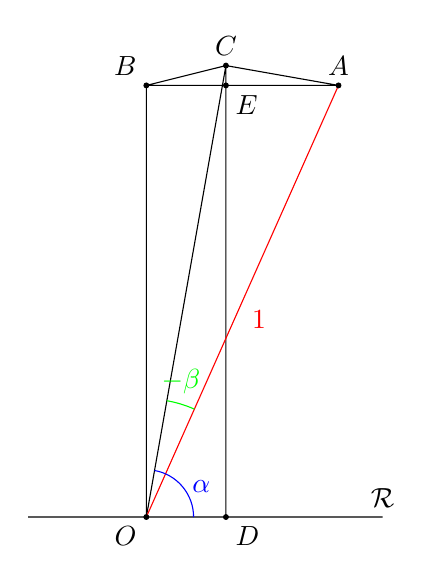
\begin{tikzpicture}
      \begin{scope}[scale=6]
        \draw (-.25,0) -- (.5,0) node[above]{$\mathcal R$}
        (0,0) -- (0,0.9135454576426009) --
        (0.4067366430758004,0.9135454576426009)

        (0.4067366430758004,0.9135454576426009) --
        (0.1684900846658375,0.9555547539512126) --
        (0,0.9135454576426009)

        (0.1684900846658375,0.9555547539512126) --
        (0.1684900846658375,0)

        (0,0)--
        (0.1684900846658375,0.9555547539512126)
        ;

        \draw[color=red]
        (0,0) --
        (0.2033683215379002,0.4567727288213004) node[below right] {$1$} --
        (0.4067366430758004,0.9135454576426009)

        ;

        \draw[fill]
        (0,0) node[below left] {$O$} circle(.005)
        (0.1684900846658375,0)
        node[below right] {$D$} circle(.005)
        (0.1684900846658375,0.9555547539512126)
        node[above] {$C$} circle(.005)
        (0,0.9135454576426009)
        node[above left] {$B$} circle(.005)
        (0.1684900846658375,0.9135454576426009)
        node[below right] {$E$} circle(.005)
        (0.4067366430758004,0.9135454576426009)
        node[above] {$A$} circle(.005)
        ;

        \draw[color=green]
         (0.0434120444167326,0.246201938253052)
         arc(80:73:.25) node[above]{$-\beta$} arc(73:66:.25);

        \draw[color=blue]
        (.1,0) arc(0:40:.1) node[right]{$\alpha$} arc(40:80:.1);


      \end{scope}
 \end{tikzpicture}
\end{center}

      We have $CO = \cos \beta$, $CA = -\sin \beta$,
  $DO = \cos \alpha \cos \beta$ and
  $DC = \sin \alpha \cos \beta$.
  In the rectangle triangle $OAB$, we now have
  $\widehat{A} = \alpha + \beta$ and so
  $BO = \sin\left(\alpha+\beta\right)$ and
  $BA = \cos\left(\alpha+\beta\right)$.
  Finally in the rectangle triangle $AEC$ we still
  have $\widehat{C} = \alpha$, $CE = -\cos \alpha \sin \beta$ and
  $EA = -\sin \alpha \sin \beta$.
  From $BO = DC - CE$ and $BA = EA + DO$ we obtain the expected formulas.

\item We have proved that the formulas hold for any
  $-\frac{\pi}{2} < \beta < 0 < \alpha < \frac{\pi}{2}$
  such that $0 < \alpha+\beta$.
  Now if $-\frac{\pi}{2} < \beta < 0 < \alpha < \frac{\pi}{2}$ and
  $\alpha+\beta < 0$ then
  $-\frac{\pi}{2} < -\alpha < 0 < -\beta < \frac{\pi}{2}$
  and $-\alpha+-\beta > 0$ so the formulas
  hold for $(-\alpha, -\beta)$. By question 7 they hold for
  $(\alpha, \beta)$.
\item Using the previous questions, we have proved that the formulas hold
  for any
  $-\frac{\pi}{2} \leq \alpha, \beta \leq \frac{\pi}{2}$. But using
  question 8, we deduce that they hold for any $\alpha, \beta$.
  The cases $\sin\left(\alpha - \beta\right)$ and
  $\cos\left(\alpha - \beta\right)$ can be derived from the expressions
  for the sum, using $\alpha - \beta = \alpha + {(-\beta)}$.
\end{enumerate}

\subsection*{Exercício 2}

\begin{enumerate}
\item We find:
    \begin{center}
    \begin{tabular}{| c | c | }
      \hline
      $x$ & $\sin{(x)}$ \\
      \hline
      $0$ & $0$ \\
      $0.15$ & $\approx 0.15$ \\
      $0.3$ & $\approx 0.30$ \\
      $0.45$ & $\approx 0.43$ \\
      $\frac{\pi}{6}$ & $\frac{1}{2}$ \\
      $0.60$ & $\approx 0.56$ \\
      $0.75$ & $\approx 0.68$ \\
      $0.90$ & $\approx 0.78$ \\
      $1.05$ & $\approx 0.87$ \\
      $1.20$ & $\approx 0.93$ \\
      $1.35$ & $\approx 0.98$ \\
      $\frac{\pi}{2}$ & $1$ \\
      \hline
    \end{tabular}
    \end{center}

  We draw the seno on $[0,\frac{\pi}{2}]$ using the values from
  the table (in red below). Since $\sin{\left(\pi-x\right)} = \sin{x}$ for all
  $x$, extend the the graph to $[0,\pi]$ (in orange). Finally, since
  $\sin{(x)} = -\sin{(x)}$ for all $x$,
  we extend the graph to $[-\pi,\pi]$ (in yellow).

  \item For all $x \in \mathbb R$, we have
    $f{\left(x+\frac{2\pi}{3}\right)} =
    2 \sin{\left(3x + 2\pi\right)} + 5 =
    2 \sin{(3x)} + 5 = f(x)$ so $f$ is $\frac{2\pi}{3}$-periodic.
    (we used $\sin{\left(y+2\pi\right)} = \sin{\left(y\right)}$)
  \item For all $x \in \mathbb R$, we have
    $\frac{f{(x)} + f{(-x)}}{2} =
    \frac{2 \sin{\left(3x\right)} + 5 +
      2 \sin{\left(-3x\right)} + 5}{2} = \frac{10}{2} = 5$
    (we used $\sin{\left(-y\right)} = -\sin{\left(y\right)}$).
    This means that $(0,5)$ is the middle of the segment delimited by the points
    $(x,f(x))$ and $(-x,f(-x))$, that is these points are symmetric with
    respect to that point. Hence $(0,5)$ is a center of symmetry of the graph
    of $f$.
  \item For all $x \in \mathbb R$, we have
    $f{\left(\frac{\pi}{3}-x\right)} =
    2 \sin{\left(\pi-3x\right)} + 5 = {2\sin{3x} +5} = f(x)
    $ (we used $\sin{(\pi-y)} = \sin{y}$).
    This means that the reta $y = \frac{\pi}{3}$ is an axis of symmetry of
    the graph of $f$.
  \item We note that the second column is the same as in the previous table.

  \begin{center}
    \begin{tabular}{| c | c | c | c | }
      \hline
      $x$ & $\sin{(3x)}$ & $2\sin{(3x)}$ & $f(x) = 2\sin{(3x)}+5$ \\
      \hline
      $0$ & $0$ & $0$ & $5$ \\
      $0.05$ & $\approx 0.15$ & $0.3$ & $5.3$ \\
      $0.1$ & $\approx 0.30$ & $0.6$ & $5.6$ \\
      $0.15$ & $\approx 0.43$ & $0.86$ & $5.86$ \\
      $\frac{\pi}{18}$ & $\frac{1}{2}$ & $1$ & $6$ \\
      $0.20$ & $\approx 0.56$ & $1.12$ & $6.12$ \\
      $0.25$ & $\approx 0.68$ & $1.36$ & $6.36$ \\
      $0.30$ & $\approx 0.78$ & $1.56$ & $6.56$ \\
      $0.35$ & $\approx 0.87$ & $1.74$ & $6.74$ \\
      $0.40$ & $\approx 0.93$ & $1.86$ & $6.86$ \\
      $0.45$ & $\approx 0.98$ & $1.96$ & $6.96$ \\
      $\frac{\pi}{6}$ & $1$ & $2$ & $7$ \\
      \hline
    \end{tabular}
  \end{center}

  We draw $f$ on $[0,\frac{\pi}{6}]$ using the values from
  the table (in blue below). Since
  $\sin{\left(\frac{\pi}{3}-x\right)} = \sin{x}$ for all
  $x$,
  extend the the graph to $\left[0,\frac{\pi}{3}\right]$ (in magenta).
  Finally, since
  $\sin{(x)} = -\sin{(x)}$ for all $x$,
  we extend the graph to $\left[-\frac{\pi}{3},\frac{\pi}{3}\right]$ (in cyan).
  We can then extend it to $\mathbb R$ using the
  $\frac{2\pi}{3}$-periodicity of $f$.

\item The graph of $x \mapsto \sin{(3x)}$ can be obtained
  horizontally shrinking the graph of $\sin$ by a factor $\frac{1}{3}$.
  The graph of $x \mapsto 2\sin{(3x)}$ can be obtained
  by vertically stretching the graph of $x \mapsto \sin{(3x)}$ by a factor $2$.
  Finally, we deduce the graph of $f$ by vertically shifting
  the graph of $x \mapsto 2\sin{(3x)}$ by $5$.

  \begin{center}
  \begin{tikzpicture}
    \draw[->] (-6,0) -- (6,0) node[above] {$x$};
    \draw[->] (0,-1.5) -- (0,8) node[right] {$y$};

    \draw[color=red]
    (0,0) --
    (0.15,0.15) --
    (0.3,0.30) --
    (0.45,0.43) --
    (0.5235987755982988,.5) --
    (0.60,0.56) --
    (0.75,0.68) --
    (0.90,0.78) --
    (1.05,0.87) --
    (1.20,0.93) --
    (1.35,0.98) --
    (1.570796326794896,1)
    ;
    \draw[color=orange]
    (3.141592653589793,0) --
    (2.991592653589793,0.15) --
    (2.841592653589793,0.30) --
    (2.691592653589793,0.43) --
    (2.617993877991494,.5) --
    (2.541592653589793,0.56) --
    (2.391592653589793,0.68) --
    (2.241592653589793,0.78) --
    (2.091592653589793,0.87) --
    (1.941592653589793,0.93) --
    (1.791592653589793,0.98) --
    (1.570796326794896,1)
    ;
    \begin{scope}[rotate=180]
    \draw[color=yellow]
    (0,0) --
    (0.15,0.15) --
    (0.3,0.30) --
    (0.45,0.43) --
    (0.5235987755982988,.5) --
    (0.60,0.56) --
    (0.75,0.68) --
    (0.90,0.78) --
    (1.05,0.87) --
    (1.20,0.93) --
    (1.35,0.98) --
    (1.570796326794896,1) --
    (1.791592653589793,0.98) --
    (1.941592653589793,0.93) --
    (2.091592653589793,0.87) --
    (2.241592653589793,0.78) --
    (2.391592653589793,0.68) --
    (2.541592653589793,0.56) --
    (2.617993877991494,.5) --
    (2.691592653589793,0.43) --
    (2.841592653589793,0.30) --
    (2.991592653589793,0.15) --
    (3.141592653589793,0)
    ;
    \end{scope}

    \foreach \i in {-2,...,2} {
    \begin{scope}[shift={(2.094395102393195*\i,5)},
                  xscale=0.3333333333333333,yscale=2]
    \draw[color=blue]
    (0,0) --
    (0.15,0.15) --
    (0.3,0.30) --
    (0.45,0.43) --
    (0.5235987755982988,.5) --
    (0.60,0.56) --
    (0.75,0.68) --
    (0.90,0.78) --
    (1.05,0.87) --
    (1.20,0.93) --
    (1.35,0.98) --
    (1.570796326794896,1)
    ;
    \draw[color=magenta]
    (3.141592653589793,0) --
    (2.991592653589793,0.15) --
    (2.841592653589793,0.30) --
    (2.691592653589793,0.43) --
    (2.617993877991494,.5) --
    (2.541592653589793,0.56) --
    (2.391592653589793,0.68) --
    (2.241592653589793,0.78) --
    (2.091592653589793,0.87) --
    (1.941592653589793,0.93) --
    (1.791592653589793,0.98) --
    (1.570796326794896,1)
    ;
    \begin{scope}[rotate=180]
    \draw[color=cyan]
    (0,0) --
    (0.15,0.15) --
    (0.3,0.30) --
    (0.45,0.43) --
    (0.5235987755982988,.5) --
    (0.60,0.56) --
    (0.75,0.68) --
    (0.90,0.78) --
    (1.05,0.87) --
    (1.20,0.93) --
    (1.35,0.98) --
    (1.570796326794896,1) --
    (1.791592653589793,0.98) --
    (1.941592653589793,0.93) --
    (2.091592653589793,0.87) --
    (2.241592653589793,0.78) --
    (2.391592653589793,0.68) --
    (2.541592653589793,0.56) --
    (2.617993877991494,.5) --
    (2.691592653589793,0.43) --
    (2.841592653589793,0.30) --
    (2.991592653589793,0.15) --
    (3.141592653589793,0)
    ;
    \end{scope}
    \end{scope}
    }

    \foreach \y in {-1,1,2,3,4,5,6,7} {
      \draw(-.1,\y) -- (.1,\y) node[right]{$\y$};
    }
    \foreach \x in {-4,-3,-2,-1,1,2,3,4} {
      \draw(\x,-.1) -- (\x,.1) node[above]{$\x$};
    }
    \draw(0,0) node [above left] {$O$};
  \end{tikzpicture}
  \end{center}

\end{enumerate}

\subsection*{Exercício 3}

\begin{enumerate}
\item For any $t$ we have
  $V(t+T) = V_0 \sin\left(2 \pi f {(t+T)}\right) =
  V_0 \sin\left(2 \pi f t + {2 \pi f T}\right)$ But
  $2 \pi f T = 2 \pi 60 \frac{1}{60} = 2 \pi$ so
  $V(t+T) = V_0 \sin\left(2 \pi f t\right) = V(t)$.

\item Depending on the are it is
  $V_0 = \sqrt{2} \times 127 \approx 179.6 \text{V}$
  or
  $V_0 = \sqrt{2} \times 220 \approx 311.1 \text{V}$.
\item We obtain the following graphs for $V_0 = 179.6 \text{V}$ (blue)
  and $V_0 = 311.1 \text{V}$ (red). We note that they have the same period
  $T = \frac{1}{60} \text{s}$ but different amplitudes.

  \begin{center}
    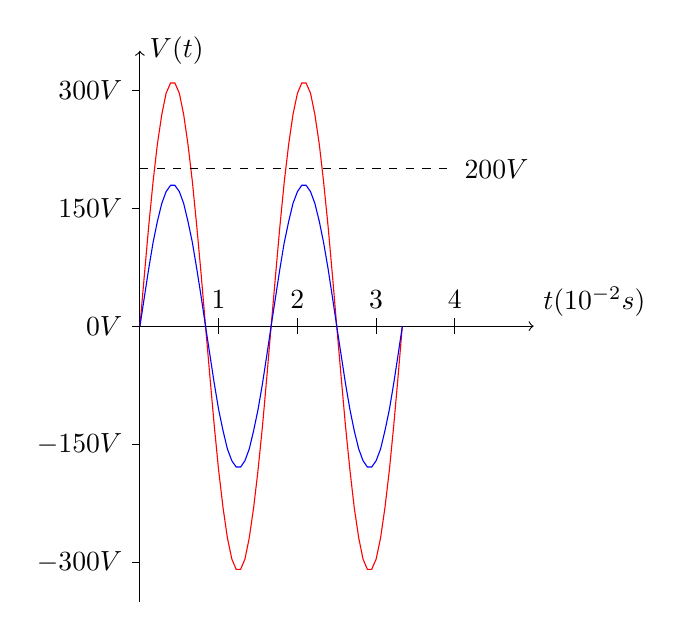
\begin{tikzpicture}
      \begin{scope}[xscale=100,yscale=.01]
    \draw[->] (0,0) -- (0.05,0) node[above right] {$t (10^{-2} \text{s})$};
    \draw[->] (0,-350) -- (0,350) node[right] {$V(t)$};
    \draw[color=red] (0,0)--(0.00056,65)--(0.00111,127)--(0.00167,183)--(0.00222,231)--(0.00278,269)--(0.00333,296)--(0.00389,309)--(0.00444,309)--(0.005,296)--(0.00556,269)--(0.00611,231)--(0.00667,183)--(0.00722,127)--(0.00778,65)--(0.00833,0)--(0.00889,-65)--(0.00944,-127)--(0.01,-183)--(0.01056,-231)--(0.01111,-269)--(0.01167,-296)--(0.01222,-309)--(0.01278,-309)--(0.01333,-296)--(0.01389,-269)--(0.01444,-231)--(0.015,-183)--(0.01556,-127)--(0.01611,-65)--(0.01667,0)--(0.01722,65)--(0.01778,127)--(0.01833,183)--(0.01889,231)--(0.01944,269)--(0.02,296)--(0.02056,309)--(0.02111,309)--(0.02167,296)--(0.02222,269)--(0.02278,231)--(0.02333,183)--(0.02389,127)--(0.02444,65)--(0.025,0)--(0.02556,-65)--(0.02611,-127)--(0.02667,-183)--(0.02722,-231)--(0.02778,-269)--(0.02833,-296)--(0.02889,-309)--(0.02944,-309)--(0.03,-296)--(0.03056,-269)--(0.03111,-231)--(0.03167,-183)--(0.03222,-127)--(0.03278,-65)--(0.03333,0);
    \draw[color=blue] (0,0)--(0.00056,37)--(0.00111,73)--(0.00167,106)--(0.00222,133)--(0.00278,156)--(0.00333,171)--(0.00389,179)--(0.00444,179)--(0.005,171)--(0.00556,156)--(0.00611,133)--(0.00667,106)--(0.00722,73)--(0.00778,37)--(0.00833,0)--(0.00889,-37)--(0.00944,-73)--(0.01,-106)--(0.01056,-133)--(0.01111,-156)--(0.01167,-171)--(0.01222,-179)--(0.01278,-179)--(0.01333,-171)--(0.01389,-156)--(0.01444,-133)--(0.015,-106)--(0.01556,-73)--(0.01611,-37)--(0.01667,0)--(0.01722,37)--(0.01778,73)--(0.01833,106)--(0.01889,133)--(0.01944,156)--(0.02,171)--(0.02056,179)--(0.02111,179)--(0.02167,171)--(0.02222,156)--(0.02278,133)--(0.02333,106)--(0.02389,73)--(0.02444,37)--(0.025,0)--(0.02556,-37)--(0.02611,-73)--(0.02667,-106)--(0.02722,-133)--(0.02778,-156)--(0.02833,-171)--(0.02889,-179)--(0.02944,-179)--(0.03,-171)--(0.03056,-156)--(0.03111,-133)--(0.03167,-106)--(0.03222,-73)--(0.03278,-37)--(0.03333,0);
    \foreach \y in {-300,-150,0,150,300} {
      \draw(0,\y) -- (-.001,\y) node[left]{$\y \text{V}$};
    }
    \foreach \x in {1,2,3,4} {
      \draw(\x/100,-10) -- (\x/100,10) node[above]{$\x$};
    }

    \draw[style=dashed](0,200)--(0.04,200) node[right]{$200 \text{V}$};
      \end{scope}
    \end{tikzpicture}
  \end{center}

\item This never happens for $127 \text{V}$ by the previous questions.
  For the other, this happens iff
  $\sin{(2 \pi f t)} = \frac{200}{\sqrt{2} V_0} = \frac{5 \sqrt{2}}{11}$
  that is
  ${\theta_0 + 2 \pi k} \leq {120 \pi t} \leq
  {\pi - \theta_0 + 2\pi k}$
  where
  $\theta_0 = \arcsin\left(\frac{5 \sqrt{2}}{11}\right)$
  and $k$ is any natural number.
  That is approximately
  $0.00185 + \frac{k}{60} \leq 0.00648 + \frac{k}{60}$
  for any natural number $k$.
\item The frequency $f' = 50\text{Hz}$ correspond to a slightly larger
  period $T'= \frac{1}{50} = 0.02\text{s}$ so the graph of $V(t)$ would
  be stretched horizontally.
\end{enumerate}

\subsection*{Exercício 4}

\begin{enumerate}
\item $x \mapsto \cos\left(x\right)$ has period $2\pi$ so
  $t \mapsto \cos\left(\omega t\right)$ has period $\frac{2\pi}{\omega}
  \approx 2\text{s}$.
\item It reaches its maximum altitude each time $\theta{(t)} = \pm 10°$ that is
  at its initial position ($t=0\text{s}$) and again every second (demi-period).
\item It reaches its minimum altitude when $\theta{(t)} = 0°$ that is the
  first time at $t=5'$ (quarter of period) and again every second (demi-period).
\item
  The altitude of the bob is $2 - \cos{\theta(t)}$ so it is less than
  $1.0038\text{m}$ iff
  $\cos{\theta(t)} \geq 0.9962$. Since ${|\theta(t)|} \leq 10°$ by assumption,
  $\cos{\theta(t)} \geq 0.9962$ is
  equivalent to ${|\theta(t)|} \leq \arccos 0.9962 \approx 5°$.
\item ${|\theta{(t)}|} \leq 5°$ is equivalent
  to $|\cos\left(\omega t\right)| \leq \frac{1}{2}$
  to ${\frac{2\pi}{3} + {2 \pi k}}
  \leq {\omega t}
  \leq {\frac{7\pi}{3} + {2 \pi k}}$ for some natural number $k$
  and finally
  ${\frac{2\pi}{3\omega} + \frac{2 \pi k}\omega}
  \leq t
  \leq {\frac{7\pi}{3\omega} + \frac{2 \pi k}\omega}$
  for some natural number $k$.
\end{enumerate}

\subsection*{Exercício 5}

\begin{enumerate}
\item This is equivalent to $\cos{u} = \pm \frac{\sqrt{3}}{2}$
  that is $u = \pm \frac{\pi}{6} + k\pi$ for $k$ any integer.
\item This is equivalent to
  $\sin{v-1} = -\frac{\sqrt{2}}{2}$ that is
  $v = 1 - \frac{\pi}{4} + 2k\pi$ and
  $v = 1 - \frac{3\pi}{4} + 2k\pi$ for $k$ any integer.
\item This is equivalent to
  $3r+2 = \frac{\pi}{2} + 2k\pi$ that is
  $r = -\frac{2}{3} + \frac{\pi}{6} + \frac{2k}{3} \pi$
  for any integer $k$.
\item This is equivalent to
  $\cos{(q-1)} = -\frac{7}{3} < -1$, which is impossible.
\item This is equivalent to
  $\tan{(h-1)} = -\frac{7}{3}$ that is
  $h = 1 - \arctan\left(\frac{7}{3}\right) + k\pi$ for any integer $k$.
\item If $X=\tan{y}$ then the equation $X^2 + {(1-\sqrt{3})} X - \sqrt{3}$
  has two solution $X=-1$ and $X=\sqrt{3}$. This corresponds to
  $y = -\frac{\pi}{4} + k \pi$ and $y = \frac{\pi}{3} + k\pi$ for any
  integer $k$.
\item We have $\sin {(3x)} +  \sin x = 2 \sin{(2x)} \cos{x}$ so the equation is
  equivalent to $\cos{x} \left(2 \sin{2x} - \sqrt{3}\right) = 0$ that is
  $\cos{x} = 0$ or $\sin{(2x)} = \frac{\sqrt{3}}{2}$. Finally the solutions are
  $\pm \frac{\pi}{2} + 2k\pi$, $\frac{\pi}{6} + k\pi$ and
  $\frac{\pi}{3} + k\pi$ for any integer $k$.
\item We have $\cos{(5t)} - \cos{(3t)} = -2 \sin{(4t)}\sin{t}$
  so the equation is equivalent to
  $\sin{t} \left(1+2\sin{(4t)}\right) = 0$
  that is $\sin{t} = 0$ or $\sin{(4t)} = -\frac{1}{2}$.
  Finally, the solutions are
  $\pm \pi + 2k\pi$,
  $\frac{-\pi}{24} + 2k\pi$ and $\frac{-5\pi}{24} + 2k\pi$ for any
  integer $k$.
\item
  We have $\cos{(2d)} = 2\cos^2{d} -1$
  so the equation is equivalent to
  $\cos^2{d} - 2\cos{d} + 1 = 0$
  that is ${(\cos{d} - 1)}^2 = 0$
  that is $\cos{d} = 1$. Hence $d = 2k\pi$ for any integer $k$.
\end{enumerate}

\subsection*{Exercício 6}

\begin{enumerate}
\item This is equivalent to $\sin{(u^2-8)} \leq \frac{4}{3}$.
  But $\sin{(u^2-8)} \leq 1 < \frac{4}{3}$ so there is no solution.
\item This is equivalent to
  $\cos{(3x - 7)} < -\frac{1}{2}$
  that is
  $\frac{2\pi}{3} + {2k\pi} < 3x - 7 < \frac{4\pi}{3} + {2k\pi}$ for some
  integer $k$ that is
  $\frac{2\pi}{9} + \frac{7+2k\pi}{3} <x< \frac{4\pi}{9} + \frac{7 + 2k\pi}{3}$
  for some integer $k$.
\item This is equivalent to ${|\sin{t}|} > \frac{\sqrt{2}}{2}$ that
  is $\frac{\pi}{4} + k\pi < t < \frac{3\pi}{4} + k\pi$ for any integer $k$.
\item This is equivalent to $\cos{(v+1)} < -\frac{7}{5} < -1$ so
   there is no solution.
 \item This is equivalent to
   $y^2-7 \in \left[{\frac{\pi}{4}+k\pi},{\frac{\pi}{2}+k\pi}\right)$
   that is
   $y^2 \in \left[{\frac{\pi}{4}+7+k\pi},{\frac{\pi}{2}+7+k\pi}\right)$
     for some integer $k$.
     We have $\frac{\pi}{2}+7+k\pi < 0$ for $k \leq -3$ and
   ${\frac{\pi}{4}+7+k\pi} > 0$ for $k \geq -2$.
     So the solutions are
     $y \in \bigcup_{{k \in \mathbb Z}, k\geq-2}
     \left[\sqrt{{\frac{\pi}{4}+7+k\pi}},
           \sqrt{{\frac{\pi}{2}+7+k\pi}}\right)$

 \item If $Y = \tan{y}$ this is equivalent to
  $Y^2 + 2Y - 63 \leq 0$. The discriminant is
  $\Delta = 256=16^2 > 0$ and the roots of the polynomial are
  $Y \in \{7, -9\}$. Hence the polynomial is $\leq 0$ iff
  $Y \in {[-9, 7]}$ that is
  $y \in \bigcup_{k \in \mathbb Z} [-\arctan{9}+k\pi,\arctan{7}+k\pi]$.
\end{enumerate}
